\graphicspath{{modelling/fig/}}
{
\tikzset{external/figure name/.add={modelling/}{}}

\chapter{Modelling}
\label{chap:modelling}

\paragraph
In this chapter, mathematical models of a multirotor with a suspended payload will be derived.
These models will be used to simulate the multirotor system in subsequent chapters.
The models will be based on the real multirotor named \emph{Honeybee}, which was built by \cite{Grobler2020} and will be described further in Chapter~\ref{chap:exp_design}.

% ?? Write this section

\paragraph
% The system identification and control system techniques in later chapters will then be explained based on the \gls{2D} model to avoid unnecessary complexity.
Finally, it will be described how this model and the techniques in later chapters are extended to the 3D case.
This 3D mathematical model will be used in a non-linear simulation of a multirotor and suspended payload.

% ?? For good modelling of multirotor, survey: https://arxiv.org/pdf/2011.11104.pdf

\FloatBarrier\section{Coordinate frames}

    \paragraph
    A quadrotor with a standard X-configuration is considered in this work.
    Figure~\ref{fig:coord_frames} shows a quadrotor schematic and two coordinate frames that will be used to describe this system.
    
    \begin{figure}[htb]
        \centering
        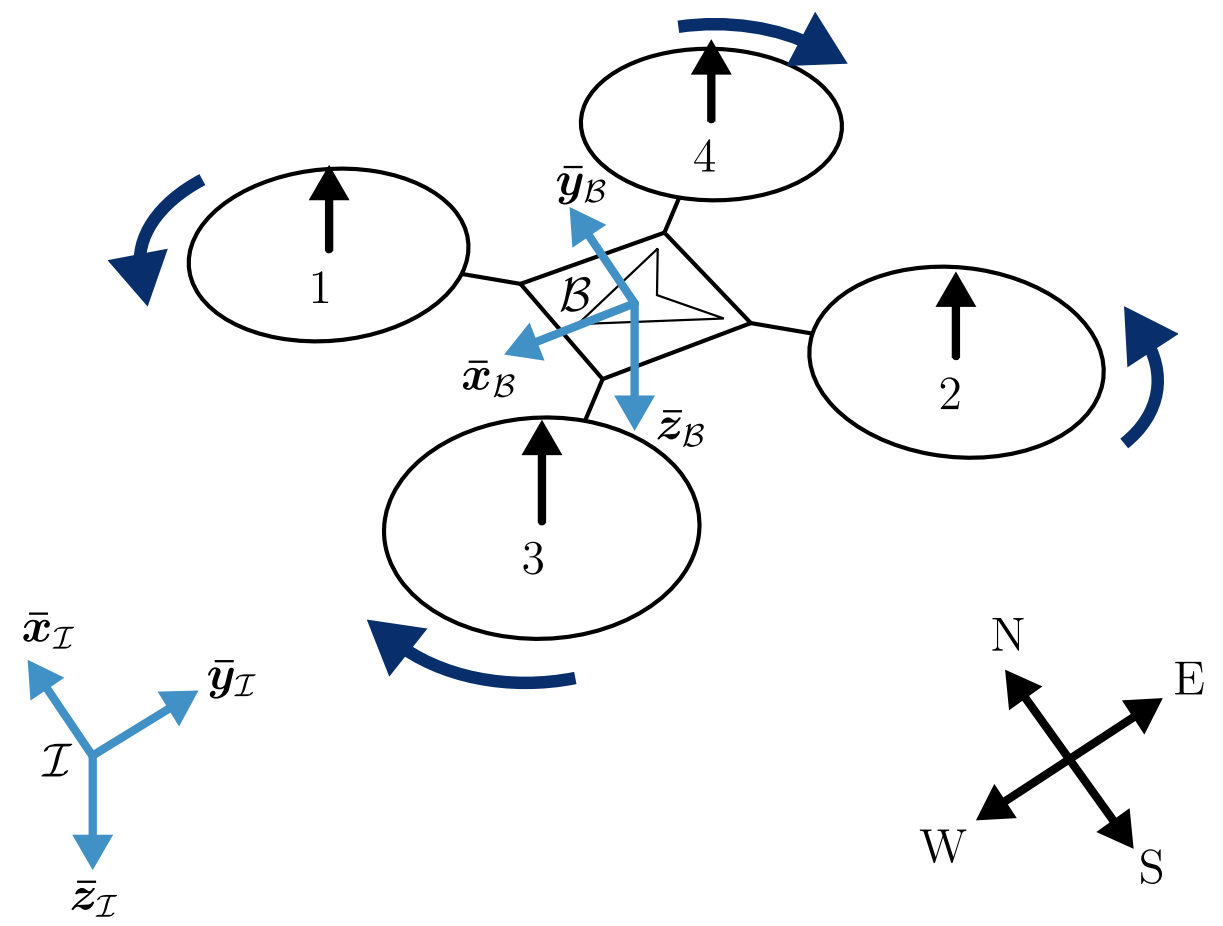
\includegraphics[width=0.6\linewidth]{modelling/fig/coord_frames}
        \caption{Inertial and body coordinate frames of a quadrotor from \cite{Erasmus2020}}
        \label{fig:coord_frames}
    \end{figure}

    \paragraph
    The inertial frame is denote by $ \mathcal{I} = \{ \bm{\bar{x}}_\mathcal{I}, \bm{\bar{y}}_\mathcal{I}, \bm{\bar{z}}_\mathcal{I} \} $ and describes a \gls{NED} axis system.
    The $x$, $y$, and $z$ axis, align with the North, East, and Down inertial directions respectively.
    The inertial frame assumes a flat, non-rotating earth, since the quadrotor will travel small distances in comparison to the curvature of the earth.
    The origin of this frame is fixed at the takeoff location of the multirotor.

    \paragraph
    The body frame is denote by $ \mathcal{B} = \{ \bm{\bar{x}}_\mathcal{B}, \bm{\bar{y}}_\mathcal{B}, \bm{\bar{z}}_\mathcal{B} \} $ and is fixed to the quadrotor body.
    The origin of this frame is at the \gls{CoM} of the vehicle and the $x$, $y$, and $z$ axis, align with the forwards, rightwards, and downwards directions of the quadrotor body respectively.
    The body frame is defined by a translation and rotation relative to the inertial frame.
    The position of the \gls{CoM} of the multirotor in the inertial frame is denoted as $P = [P_N~~P_E~~P_D]^T$. 
    This represents the translation of the body frame relative to the inertial frame.
    The rotations will be discussed in the section below.

\FloatBarrier\section{Rotations}
    
    \paragraph
    The rotation of the body frame relative to the inertial frame can also be referred to as the attitude of the multirotor.
    This can be defined in terms of Euler angles or quaternions.

    \FloatBarrier\subsection{Euler angles}

        \paragraph
        Euler angles are a popular way of describing a \gls{3D} rotation as a sequence of three consecutive elementary rotations \cite{Brescianini2013}.
        For aircraft applications, the ZYX-sequence is common \cite{Brescianini2013} and will be used in this work.
        The order of rotations are:
        \begin{enumerate}
            \item Rotate the body frame about the $z$-axis by the yaw angle, $\Psi$.
            \item Rotate the resulting frame about the new $y$-axis by the pitch angle, $\Theta$.
            \item Rotate the resulting frame about the new $x$-axis by the roll angle, $\Phi$.
        \end{enumerate}

        \begin{figure}[!htbp]
            \centering
            \vspace{0.5cm}
            \def\svgwidth{\columnwidth}
            \scalebox{1.0}{\input{modelling/fig/Euler_rotations.pdf_tex}}
            \caption{Illustration of Euler angles from \cite{Slabber2020}}
            \label{fig:Euler_rotations}
        \end{figure}

        \paragraph
        Figure~\ref{fig:Euler_rotations} gives a simple illustration of the Euler ZYX angles.
        Note that $\Theta$ and $\Phi$ are each illustrated as a pure pitch angle and roll angle from the the inertial frame, without a prior Euler rotation.

    \FloatBarrier\subsection{Quaternions}

        \paragraph
        introduce


\FloatBarrier\section{Multirotor with a suspended payload}

    \paragraph
    The suspended payload is modelled as a rigid body attached by a link to the \gls{CoM} of the quadrotor rigid body.
    Figure~\ref{fig:quad_payload} illustrates a quadrotor with a suspended payload.
    The Euler ZYX angles of the suspended payload in the inertial frame are also shown.
    The $x$-axis and $y$-axis Euler angles are denoted by $\theta_p$ and $\phi_p$ respectively.
    The $z$-axis Euler angle does not contribute to the system dynamics and is omitted. 

    \begin{figure}[!htbp]
        \centering
        \def\svgwidth{\columnwidth}
        \scalebox{0.6}{\input{modelling/fig/quad_payload.pdf_tex}}
        \caption{Schematic of a quadrotor with suspended payload from \cite{Slabber2020}}
        \label{fig:quad_payload}
    \end{figure}
    
    The following assumptions are made regarding the payload model:
    \begin{itemize}
        \item The payload is a point mass.
        \item The link is massless.
        \item The link is rigid.
        \item The link is attached to the \gls{CoM} of the multirotor.
    \end{itemize}

    \paragraph
    The payloads used in the practical setup and described in Chapter~\ref{chap:exp_design}, 
    are small relative to the quadrotor and the attachment point is close to the payload \gls{CoM}.
    They are attached with a low-friction swivel to the suspended cable, therefore the rotation of the payload around the cable axis has a negligible effect on the quadrotor. 
    Therefore modelling a payload as a point mass seems reasonable.

    \paragraph
    The cables used in Chapter~\ref{chap:exp_design} have a very low mass in comparison to the payloads and have a negligible amount of stretch.
    Furthermore, the cable remains straight and rigid during flight due to the tension applied by the payload.
    Aggressive flights may cause periods of zero cable tension where the load is in free-fall and the cable is slack \cite{Tang2015}.
    However, such aggressive manoeuvres will not be considered in this work and the assumption of a rigid, massless cable appears reasonable.

    \paragraph
    In the practical setup shown in Chapter~\ref{chap:exp_design}, the cable is attached appears to be very near to the \gls{CoM} of the quadrotor.
    It is assumed that if the attachment point is slightly below this point it will have a negligible effect on the dynamics.

\FloatBarrier\section{Forces and moments}

    \paragraph
    damping of payload angle


\FloatBarrier\section{Lagrangian mechanics}
    \begin{enumerate}
        \item Discuss weak link between altitude dynamics and swing angle
    \end{enumerate}


\FloatBarrier\section{Model verification} \label{sec:model_verification}

    \paragraph
    Intro

    \begin{figure}[htb]
    \centering
    \begin{tikzpicture}
        \begin{axis}[            
            xlabel = Time,
            ylabel = North velocity,
            x unit = \si{\second},
            y unit = \si{\metre/\second},
            xmin = 0,   xmax = 16,
            ymin = -0.1,  ymax = 2.5,
            grid = major,
            legend cell align = left,
            legend pos = south east,
            grid style = dashed,
            legend style = {font = \scriptsize},
            label style = {font = \scriptsize},
            tick label style = {font = \scriptsize},
            width = 0.95\columnwidth,
            height = 0.5\columnwidth,
            % initialize Dark2
            cycle list/Dark2,
            % combine it with 'mark list*':
            cycle multiindex* list = {
                Dark2\nextlist
            }
        ]
                
        \addplot+[mark = none, style = solid, ultra thick] 
        table[x = time, y = vel_sp, col sep = comma] 
        {modelling/csv/prac_vs_sim_vel_step_Simulink_2021-08-20_04_no_load_velocity_steps_wind_0.5.csv.csv};
        \addlegendentry{$V_{N_{sp}}$}

        \addplot+[mark = none, style = solid, ultra thick] 
        table[x = time, y = vel.prac, col sep = comma] 
        {modelling/csv/prac_vs_sim_vel_step_Simulink_2021-08-20_04_no_load_velocity_steps_wind_0.5.csv.csv};
        \addlegendentry{$V_N$ (Practical)}

        \addplot+[mark = none, style = dashed, ultra thick] 
        table[x = time, y = vel.sim, col sep = comma] 
        {modelling/csv/prac_vs_sim_vel_step_Simulink_2021-08-20_04_no_load_velocity_steps_wind_0.5.csv.csv};
        \addlegendentry{$V_N$ (Simulated)}

        \end{axis}
    \end{tikzpicture} 
    \caption{Comparison of simulated and practical data from Honeybee.}
    \label{fig:prac_vs_sim_vel_step_no_payload}
\end{figure}


    \paragraph
    No load

    \begin{figure}[htb]
    \centering
    \begin{tikzpicture}
        \begin{axis}[            
            xlabel = Time,
            ylabel = North velocity,
            x unit = \si{\second},
            y unit = \si{\metre/\second},
            xmin = 0,   xmax = 16,
            ymin = -0.1,  ymax = 2.8,
            grid = major,
            legend cell align = left,
            legend pos = south east,
            grid style = dashed,
            legend style = {font = \scriptsize},
            label style = {font = \scriptsize},
            tick label style = {font = \scriptsize},
            width = 0.95\columnwidth,
            height = 0.5\columnwidth,
            % initialize Dark2
            cycle list/Dark2,
            % combine it with 'mark list*':
            cycle multiindex* list = {
                Dark2\nextlist
            }
        ]
                
        \addplot+[mark = none, style = solid, ultra thick] 
        table[x = time, y = vel_sp, col sep = comma] 
        {modelling/csv/prac_vs_sim_vel_step_Simulink_2021-08-20_02_l-2_mp-0.3-wind-0.5.csv.csv};
        \addlegendentry{$V_{N_{sp}}$}

        \addplot+[mark = none, style = solid, ultra thick] 
        table[x = time, y = vel.prac, col sep = comma] 
        {modelling/csv/prac_vs_sim_vel_step_Simulink_2021-08-20_02_l-2_mp-0.3-wind-0.5.csv.csv};
        \addlegendentry{$V_N$ (Practical)}

        \addplot+[mark = none, style = dashed, ultra thick] 
        table[x = time, y = vel.sim, col sep = comma] 
        {modelling/csv/prac_vs_sim_vel_step_Simulink_2021-08-20_02_l-2_mp-0.3-wind-0.5.csv.csv};
        \addlegendentry{$V_N$ (Simulated)}

        \end{axis}
    \end{tikzpicture} 
    \caption{Velocity step comparison of simulated and practical data for Honeybee with a suspended payload.}
    \label{fig:prac_vs_sim_vel_step_with_payload}
\end{figure}


    \paragraph
    With payload vel

    \begin{figure}[htb]
    \centering
    \begin{tikzpicture}
        \begin{axis}[            
            xlabel = Time,
            ylabel = Payload angle,
            x unit = \si{\second},
            y unit = \si{\degree},
            xmin = 0,   xmax = 16,
            ymin = -20,  ymax = 20,
            grid = major,
            legend cell align = left,
            legend pos = south east,
            grid style = dashed,
            legend style = {font = \scriptsize},
            label style = {font = \scriptsize},
            tick label style = {font = \scriptsize},
            width = 0.95\columnwidth,
            height = 0.5\columnwidth,
            % initialize Dark2
            cycle list/Dark2,
            % combine it with 'mark list*':
            cycle multiindex* list = {
                Dark2\nextlist
            }
        ]
                
        \addplot+[mark = none, style = solid, ultra thick] 
        table[x = time, y = theta.prac, col sep = comma] 
        {modelling/csv/prac_vs_sim_vel_step_Simulink_2021-08-20_02_l-2_mp-0.3-wind-0.5.csv.csv};
        \addlegendentry{Practical}

        \addplot+[mark = none, style = dashed, ultra thick] 
        table[x = time, y = theta.sim, col sep = comma] 
        {modelling/csv/prac_vs_sim_vel_step_Simulink_2021-08-20_02_l-2_mp-0.3-wind-0.5.csv.csv};
        \addlegendentry{Simulated}

        \end{axis}
    \end{tikzpicture} 
    \caption{Payload angle comparison of simulated and practical data for Honeybee with a suspended payload}
    \label{fig:prac_vs_sim_theta_with_payload}
\end{figure}


    \paragraph
    With payload theta



    \begin{enumerate}
        \item Plot velocity step
        \item Plot position step
    \end{enumerate}

\FloatBarrier\section{Linearised model}
    \label{sec:linear_model}

\FloatBarrier\section{Dynamic payloads}

    In this work, a dynamic payload refers to a payload with dynamics that differ significantly from a rigid mass.
    When considering suspended payloads, a dynamic payload induces dynamics which differ from that of a simple pendulum.

    \begin{itemize}
        \item Most control in literature model payload as rigid Mass. Give references.
        \item Some add spring stiffness of cable (give references e.g. QuadLoad ElasticCable Prasanth Kotaru)
        \item but not practical because can design which cable you used. Cannot design which payload needs to be transported
        \item water looks like double payload
    \end{itemize}
% https://hybrid-robotics.berkeley.edu/publications/ACC2017_QuadLoad_ElasticCable.pdf), 
% https://www.researchgate.net/publication/352394086_A_Hybrid_Control_Approach_for_the_Sw[…]=publicationTitle&_iepl%5BtargetEntityId%5D=PB%3A352394086

}

